\documentclass[output=paper]{langsci/langscibook}

\author{Aritz Irurtzun\affiliation{CNRS-IKER (UMR 5478)}}
\title{Revisiting the lack of verbal \textit{wh}-words}

% \chapterDOI{} %will be filled in at production

\abstract{I propose that the cross-linguistic lack of verbal \emph{wh}-words
    derives from the ill-formed \gls{LF} representations they would generate: verbs
    are predicates of eventualities and predication ($\approx$logical
    attribution) and questioning are incompatible. I revisit the literature on
    interrogative \isi{pro-verbs} arguing that there are no genuine interrogative
    verbs unrestrictedly ranging over any eventuality type. Last, I argue that
    my proposal also predicts the universal lack of other conceivable
interrogative elements such as adpositions or tense markers.}

\maketitle

\begin{document}\glsresetall

\section{Impossible questions}

One of the prima facie most puzzling cross-linguistic constraints is the
apparent lack of genuine verbal \emph{wh}-words\is{wh-words!verbal wh-words} asking about the nature of the
eventuality at stake.

For an illustration, let us take a situation like the one in Figure 1, the
assassination of Julius C\ae{}sar (as depicted in the 1798 painting by Vincenzo
Camuccini).

\begin{figure}[H]
\centering
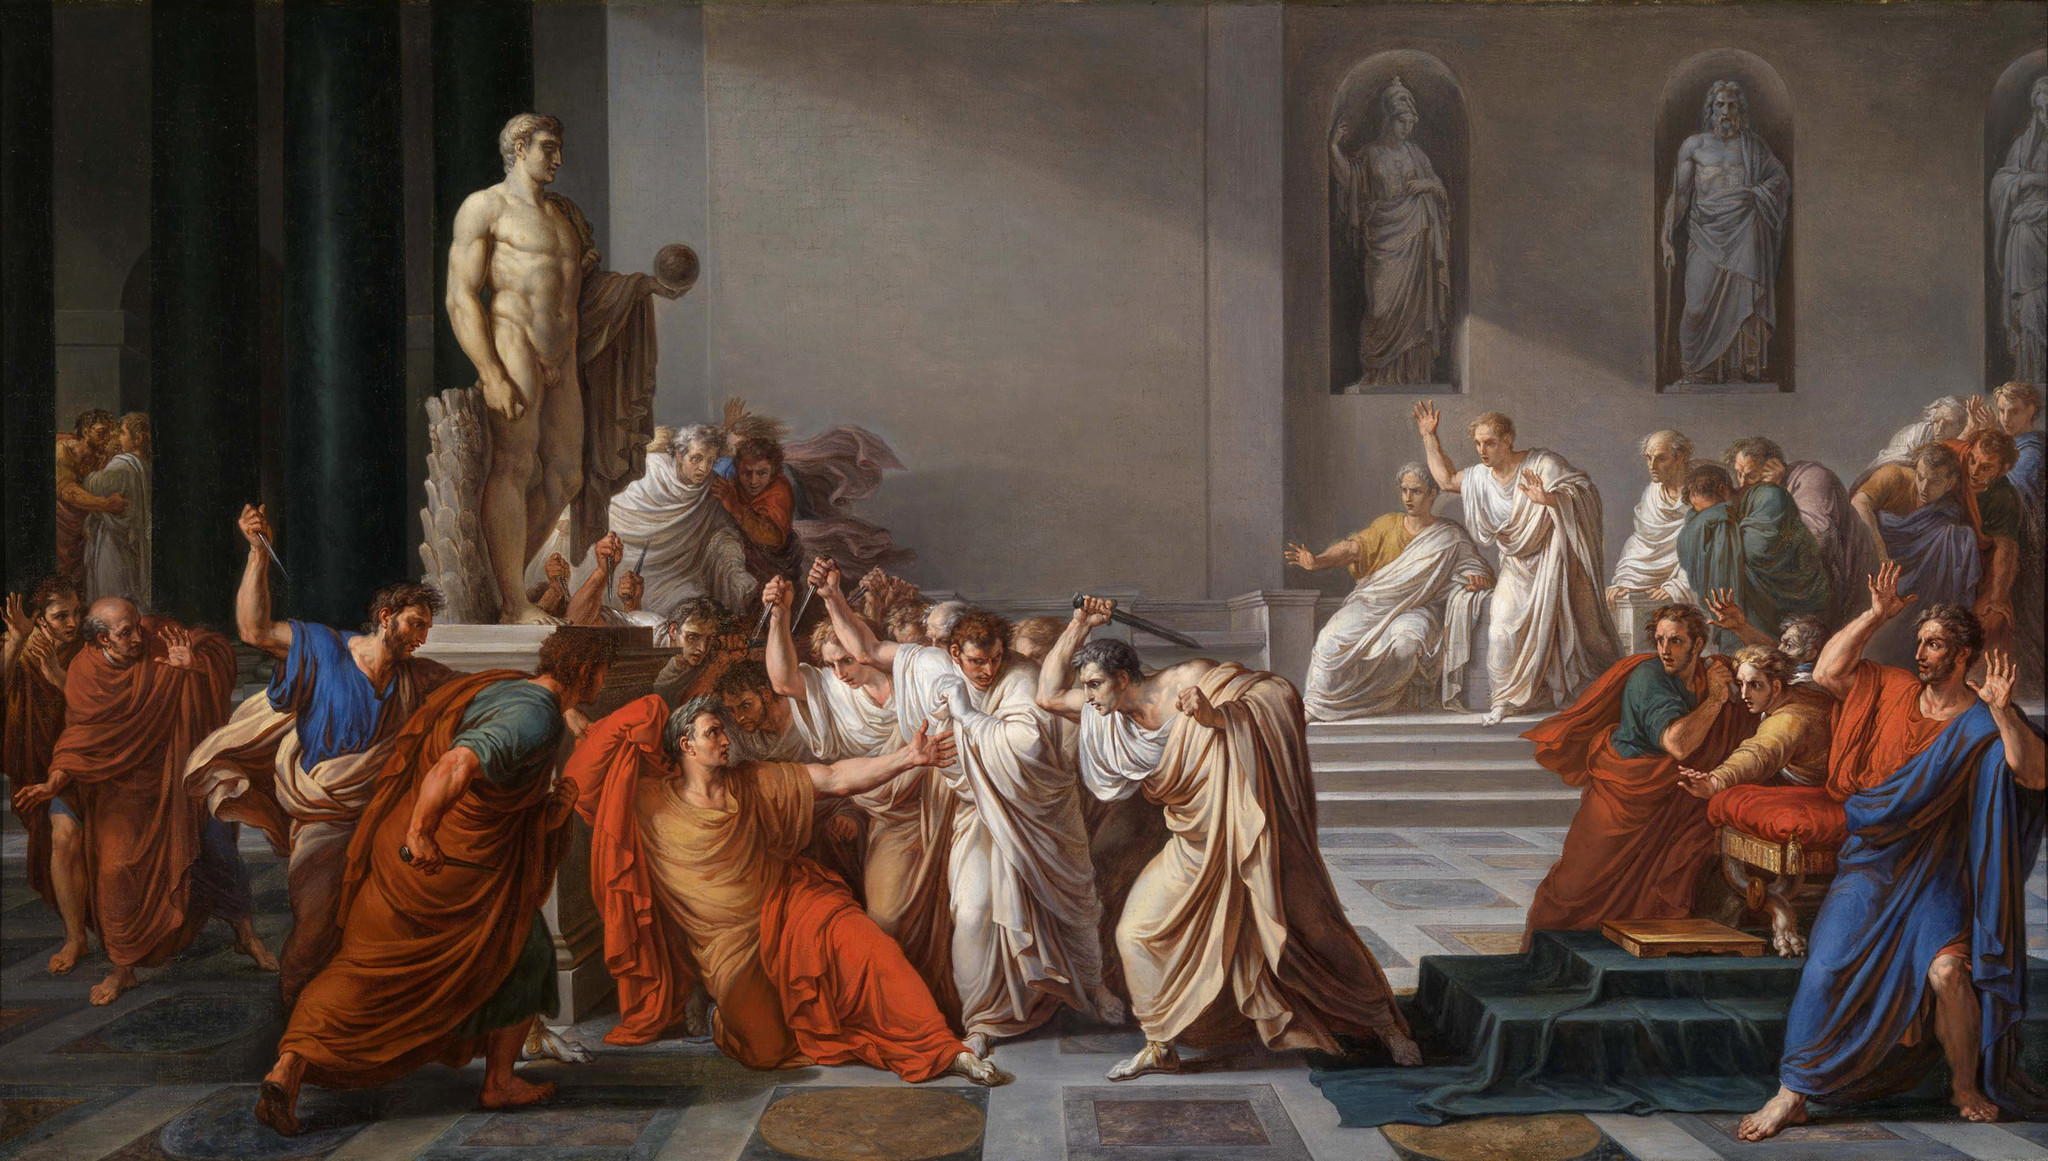
\includegraphics[width=.8\textwidth,keepaspectratio=true]{./img/15.png}
\caption{\emph{La morte di Cesare} (V. Camuccini)}
\end{figure}

Such an event can be described with the proposition expressed by (\ref{one}), a
classic example discussed by \citet{Davidson1967} and many others:

\begin{exe}
\ex \label{one} Brutus stabbed C\ae{}sar.
\end{exe}

But besides asserting what happened, there is a variety of questions we may ask
about the event: questions about the killer (\ref{1}), the killed one
(\ref{2}), the location of the event (\ref{3}), the moment that it took place
(\ref{4}), the way it was performed (\ref{5}), or the motives of the assassin
(\ref{6}), among others:

\begin{exe}
\ex \label{1} \emph{Who} stabbed C\ae{}sar?
\ex \label{2} \emph{Whom} did Brutus stab?
\ex \label{3} \emph{Where} did Brutus stab C\ae{}sar?
\ex \label{4} \emph{When} did Brutus stab C\ae{}sar?
\ex \label{5} \emph{How} did Brutus stab C\ae{}sar?
\ex \label{6} \emph{Why} did Brutus stab C\ae{}sar?
\end{exe}

All of them are perfectly grammatical questions. However, there is a type of
question that we cannot directly ask; we cannot ask questions on the nature of
the eventuality itself. There is simply no interrogative pro-verb, so that we
can ask questions such as (\ref{7}):

\ea[*]{\emph{Whxyzed} Brutus C\ae{}sar?\\
    `What type of event happened such that it has Brutus as external argument
and C\ae{}sar as internal argument?'}\label{7}
\z

We could generalize this observation as in (\ref{gen}):

\ea
\label{gen}
\emph{Generalization}: There are no verbal \emph{wh}-words\is{wh-words!verbal wh-words} ranging over any
eventuality type.\footnote{See \Cref{sec:revisiting} for discussion.}
\z

This is such an obvious fact that it has seldom been discussed in linguistics
(see a few exceptions in
\citealt{hagege2003,hagege2008,cysouw2004,idiatov.vanderauwera2004}).

The way many languages (including English) have of circumventing the lack of
verbal \emph{wh}-words\is{wh-words!verbal wh-words} is to decompose the transitive pro-verb of (\ref{7})
into a dummy \emph{do} verb and an interrogative pronoun as its direct
object, as in (\ref{8}):\largerpage[1]

\ea
\label{8} \emph{What} did Brutus \emph{do} to C\ae{}sar?
\z

In this article, I discuss the nature and strength of this constraint and
propose a formal account for it based on general legibility constraints
(representational well-formedness conditions) at the interface between language
and the conceptual--intentional (C--I) systems which would be violated by genuine
interrogative \isi{pro-verbs}. After briefly discussing the cross-linguistic
availability of interrogative \isi{pro-verbs} in \Cref{sec:2}, in \Cref{sec:3} I make
the proposal that the lack of verbal \emph{wh}-words\is{wh-words!verbal wh-words} is due to the fact that
sentences with genuine interrogative \isi{pro-verbs} would generate ill-formed
logical forms for the C--I interface. In \Cref{sec:revisiting} I revisit the
evidence for interrogative \isi{pro-verbs} in the light of my proposal and in
\Cref{sec:prediction} I briefly address a prediction my proposal makes
regarding the unavailability of other conceivable \emph{wh}-words such as
interrogative adpositions or tense markers.\is{wh-words}\largerpage[-1]

\section{A marked cross-linguistic option} \label{sec:2}

The lack of verbal \emph{wh}-words\is{wh-words!verbal wh-words} is a cross-linguistically pervasive
phenomenon to the point that \citet{hagege2003} questions ``Whatted we to
interrogative verbs?'' as a way of expressing the typological rarity of them
(see also \citealt{hagege2008,idiatov.vanderauwera2004} for further
typological analyses).\footnote{Actually, in \ili{Basque} (isolate), as in other
    languages, there is the morphological equivalent of
    \citeauthor{hagege2003}'s \citeyearpar{hagege2003} ``whatted'',
    \emph{zertu}, which is composed of the indefinite/interrogative pronoun
    \emph{zer} and the verbalizer suffix \emph{-tu}. This verb, however,
    does not have the value of an interrogative pro-verb, but that of a
    ``regular'' pro-verb (that of avoiding to lexically express the nature of an
    eventuality, typically because of word retrieval difficulties, or because
    we want to avoid being too explicit about it (because of taboo or so)).

%Aizu, ordea: ba al dakizu zuk beribilla zertzen? —Ez nik; ez dakit. (Eusebio Erkiaga, \emph{Araibar zalduna} (1962))
\label{fn:15.2}}

In what is probably the broadest comparative analysis so far,
\citet{hagege2008} studies a sample of 217 languages of which he only
classifies 28 as having the property of displaying interrogative \isi{pro-verbs}. He
conjectures that this may be due to an economy restriction against
morphologically unanalyzable forms:

\begin{quote}This suggests that if interrogative verbs
are found in so few languages, one of the reasons might be that most of them
use an uneconomical device, by saying `do what’, for example, in a single
unanalyzable unit, instead of using a succession of two very frequent elements,
meaning, respectively, `do’ and `what’.\hfill \citep[30]{hagege2008}
\end{quote}

I believe that this cannot be the reason for their scarcity, for otherwise
decomposed \emph{wh}-words\is{wh-words} (\emph{what person} = who, \emph{what place}
= where, \emph{what time} = when, etc.) would be the norm across natural
languages. And languages would resemble each other much more in this
respect.\footnote{Alternatively, \citet{idiatov.vanderauwera2004} hypothesize
    that \emph{wh}-questions involve an existential presupposition such as
    (i):

\begin{exe}
\exi{(i)} \label{i} A constituent question is a question that asks for an
instantiation of the variable $x$ in an ``It is known that (possibly) \textsc{happen}\slash\textsc{exist}%
(\dots{} $x$ \dots{})'' structure.
\end{exe}
According to their analysis, such a structure would be the presupposition that
the situation under interrogation (possibly) exists, existed or will exist, and
the variable \emph{x} is formally expressed by an interrogative pro-word. They
conjecture that only ``endocentric phrasal'' elements can be \emph{wh}-words\is{wh-words} but such an analysis is also problematic, since it implies that all \emph{wh}-words are phrasal, and that verbs are simple terminal elements, contrary to standard analyses of argument structure (see below).}
In the next section I will make an alternative proposal (a formal one) trying
to account for this typological puzzle claiming that genuine interrogative
pro-verbs (verbs asking about eventuality types) cannot exist because they
would violate legibility constraints at the C--I interface.

\section{A conjecture: Illegibility at the conceptual--intentional
interface}\label{sec:3}

I would like to propose that the lack of verbal \emph{wh}-words\is{wh-words!verbal wh-words}
cross-linguistically derives from a legibility constraint at the interface
between the linguistic computation and the language-external
conceptual--intentional systems (by assumption, universal across the species).
The idea is that C--I systems impose legibility well-formedness conditions on
their possible inputs (namely, on the form of acceptable logical form
representations) and the logical forms corresponding to sentences including
genuine interrogative \isi{pro-verbs} would violate those legibility constraints.
Thus, if my hypothesis is correct, the general lack of verbal \emph{wh}-words\is{wh-words!verbal wh-words}
is an interesting fact about languages, but not a linguistic fact in essence
(for it derives from conditions imposed onto language by language-external
systems of thought).\footnote{See
\citet{Chomsky2005,BerwickEtAl2011,Roberts2012,biberauer.roberts2017} for
discussion on the different factors affecting the design features of
I-languages.}

In particular, my proposal is that the lack of interrogative verbs derives from
a general constraint on the logic of \isi{predication}: predication amounts to
logical assertion whereby a property is ascribed/attributed/applied to an
object (cf.\ i.a.
\citealt{engel1989,parteeetal1990,mcginn2000,davidson2005,burge2007,liebesman2015}).
That is, predicates predicate and it is therefore that predication qua
interrogation is incongruent (not only in first-order logic).\newpage

Furthermore, I shall argue that an ``interrogation qua \isi{predication}''
would also derive into having logical form representations with DPs devoid of
θ-roles (violating the θ-criterion,  cf.
\citealt{Chomsky1981} or \citealt{Higginbotham1985}).

To begin with, it is essentially a truism that argument DPs function as
participants in the eventuality denoted by the verb in a clause. Semanticists
and philosophers of language have distinguished different types of
participation (the literature talks about agents, themes, undergoers,
experiencers, beneficiaries, etc. as the potential thematic- (or θ-)
roles that a verbal argument can have) and the existence of some sort of
θ-roles is virtually undisputed in linguistic theory, even if their
conception and ontological status varies from one work to the other (see
e.g.\ \citealt{carlson1984,Dowty1989,parsons1995}). A more
``syntacticising'' view of θ-roles\is{thematic roles} even proposes that θ-roles
should be syntactically conceived as formal features, with a legibility
requirement that those features be derivationally checked by \gls{LF} (see
i.a.\
\citealt{boskovic.takahashi1998,hornstein1999,lasnik1999,manzini.roussou2000,fanselow2001,bagchi2007}).\footnote{In
    the P\&P framework, the projection principle guaranteed all
    argument-structure restrictions to be set at D-Structure, but with the
    minimalist abandonment of internal levels of representation, an option
    opened for not all argument-structure relations to be set at first merge,
    therefore allowing for movement into θ-positions (see the references
above).}

In particular, θ-roles\is{thematic roles} are central to neo-Davidsonian semantics, a
conception of semantics deeply rooted in the philosophy of language that
constitutes a natural partner of minimalist syntax (see
\citealt{Parsons1990,parsons1995,herburger2000,hornstein2002,pietroski2002,pietroski2003,pietroski2005,schein2002,irurtzun2007,Lohndal2014}).
In this framework, θ-roles\is{thematic roles} function as the link between arguments and
events in logical form. For instance, example (\ref{one}) -- repeated here as
(\ref{dav1}) -- would have the neo-Davidsonian logical form representation in
(\ref{dav2}), which roughly reads as ``there was an event that was a stabbing
event that is past and whose agent was Brutus and whose patient was
C\ae{}sar'':

\begin{exe}
\ex
\begin{xlista}
\ex \label{dav1} Brutus stabbed C\ae{}sar.
\ex \label{dav2} $\exists$e [Agent(e, Brutus) \& Stabbing(e) \& Past(e) \& Patient(e, C\ae{}sar)]
\end{xlista}
\end{exe}

The nature of each θ-role\is{thematic roles} directly derives from the bottom-up syntactic
composition of the clause, whereby DPs are merged in specific positions within
the projection of event-denoting heads (see i.a.\
\citealt{pietroski2003,pietroski2005,Borer2005,Ramchand2008}).

I would like to propose that the requirement for DPs to bear θ-roles
derives precisely from the neo-Davidsonian logical form representation of
sentences at the C--I interface: as shown in (\ref{dav2}) θ-roles\is{thematic roles} relate
individuals and eventualities and my proposal is that \emph{wh}-words\is{wh-words}
introduce variables that may range over individuals, as in (\ref{dav3}), for
`Who stabbed C\ae{}sar?', or (\ref{dav4}), for `Whom did Brutus stab?', or
other elements like adjuncts (see below \Cref{sec:prediction}), but
\emph{not} over predicates of eventualities. As a matter of fact, predicating
an interrogation is logically incongruent for predicates
\emph{assert/attribute} and interrogations \emph{query}
(\ref{dav5}):\footnote{For simplicity, I stick to this declarative type of
logical form representation; see in \citet{lohndal.pietroski2011} an approach
to an ``I-Semantics'' for questions.}

\begin{exe}
\ex
\begin{xlista}
\ex[]{$\exists$e [Agent(e, ?) \& Stabbing(e) \& Past(e) \& Patient(e, C\ae{}sar)]}\label{dav3}
\ex[]{$\exists$e [Agent(e, Brutus) \& Stabbing(e) \& Past(e) \& Patient(e, ?)]}\label{dav4}
\ex[*]{$\exists$e [Agent(e, Brutus) \& ?(e) \& Past(e) \& Patient(e, C\ae{}sar)]}\label{dav5}
\end{xlista}
\end{exe}

That is, the logical form in (\ref{dav5}) involves a predicate that questions
its own essence, and this is incompatible with the essential function of a
predicate: predicating (i.e. ascribing properties).

Furthermore -- and this is important (see~\Cref{sec:revisiting}) -- a
logical form along the lines in (\ref{dav5}) would still be unwarranted. In
fact, a predicate like \emph{?(e)} crucially devoids the eventuality of any
nature (it is completely undetermined), and as a consequence the DPs
participating in the eventuality get no θ-role\is{thematic roles} (given that
θ-roles directly depend on the nature/structure of the eventuality at
stake). In other words, in the absence of a specific semantic (and structural)
specification for the verbal predicate of eventualities, its arguments will
also be devoid of any θ-role\is{thematic roles}, since θ-role\is{thematic roles} assignment directly
depends on the structure at the \emph{v}P layer.\footnote{In particular,
    decompositional analyses such as \citeauthor{Ramchand2008}'s
    \citeyearpar{Ramchand2008} propose that verbal predicates are phrases that
    may be composed by different heads (Initiationº, Processº, Resultº) ordered
    in the hierarchical embedding relation of sub-events and that the
    θ-role\is{thematic roles} that a DP will get directly depends on the position where it
    was merged:

\begin{tikzpicture}[sibling distance=2pt]
\tikzset{level distance=24pt}
\tikzset{every tree node/.style={align=center,anchor=north}}
\begin{small}
 \Tree [.{\emph{init}P}
 {DP3\\ \begin{small}{subj of `cause'}\end{small}}				[.{\emph{init'}}
 \emph{init} 			[.\emph{proc}P 	{DP2\\ \begin{small}{subj of `process'}\end{small}}	[.{\emph{proc'}}  \emph{proc}	[.\emph{res}P		{DP1\\ \begin{small}{subj of `result'}\end{small}}	[.{\emph{result'}}	\emph{res}	XP	]]]]]]
\end{small}
\end{tikzpicture}}

Thus, rather than (\ref{dav5}), the consequence of having an
\enquote{interrogation-cum-pre\-di\-ca\-tion} would be along the lines
in (\ref{dav6}), where \underline{\hspace{1cm}} represents the unassigned
θ-roles of the participants:

\begin{exe}
\ex[*]{\label{dav6}$\exists$e [ \underline{\hspace{1cm}}(e, Brutus) \& ?(e) \& Past(e) \& \underline{\hspace{1cm}}(e, C\ae{}sar)]}
\end{exe}

Note that something like (\ref{dav6}) is not a mere instance of structural
ambiguity vis-\'a-vis the hearer; but an instance of
\emph{structural vagueness} and therefore, of ungrammaticality (cf.
the θ-criterion). An underspecified representation such as (\ref{dav6})
would generalize over all sorts of argument structures with different
θ-role assignments; from \emph{Brutus stabbed C\ae{}sar}, to
\emph{Brutus liked C\ae{}sar}, \emph{Brutus had C\ae{}sar}, \emph{Brutus
obtained C\ae{}sar}, \emph{Brutus created C\ae{}sar}, \emph{Brutus became
C\ae{}sar}, or \emph{Brutus was C\ae{}sar}.

Again, the way \ili{English} (and many other languages) has to circumvent the lack of
verbal \emph{wh}-words\is{wh-words!verbal wh-words} is to employ a complex \emph{do what} predicate that
introduces a direct object and implies the assignment of an Agent θ-role\is{thematic roles} to the
subject. This, of course, results in a convergent logical form representation.
In contrast, the logical form in (\ref{dav6}) is critically underdetermined
where \emph{\underline{\hspace{1cm}}(e, Brutus/C\ae{}sar)} may correspond to
any theta role (agent, experiencer, possessor, \ldots). In fact, there is no neat
way of expressing such a meaning in plain \ili{English} (which is precisely my point)
but it would correspond to some higher-order description including
metalinguistic terms along the lines already expressed in (\ref{7}), here
modified to (\ref{HighOrd}):

\begin{exe}
\ex \label{HighOrd} Meaning of (\ref{dav6}): `What type of eventuality happened such that it has Brutus as external argument (whatever the θ-role) and C\ae{}sar as internal argument (whatever the θ-role)?'
\end{exe}

The fact that the assignment of θ-roles\is{thematic roles} depends on the structure of the sentence, and that different θ-roles\is{thematic roles} depend on different syntactic configurations makes clear that questions such as (\ref{7}) or (\ref{dav6}) cannot exist in natural language.

In a nutshell then, my proposal is the following one:

\begin{exe}
\ex \label{prop} \emph{Proposal:} The lack of verbal question-words derives
from the illegibility they would generate at the C--I interface, since their semantics involves predicating interrogations and a failure to assign θ-roles\is{thematic roles} to event participants.
\end{exe}

In the next section I revisit the cross-linguistic evidence for interrogative
pro-verbs arguing that a large number of the ``interrogative verbs'' purported in the literature do not question the type of eventuality itself, and the few cases that actually do so are loaded semantically, so that specific event structures and θ-roles\is{thematic roles} (or macro-roles) are established.

\section{Revisiting the evidence}
\label{sec:revisiting}

The hypothesis I just presented predicts the lack of \emph{wh}-words that
question the nature of an eventuality. However, note that it leaves room for
verbal \emph{wh}-words\is{wh-words!verbal wh-words} to exist, provided that they are semantically ``loaded''
(the type of eventuality they stand for is determinate and so are the θ-roles
of their participants). In this section, I will argue that this prediction is
borne out and that the few predicates questioning the nature of the eventuality
that are found cross-linguistically are of this sort: they are not agnostic as
to the type of eventuality which is at stake.

In this section, I review the evidence for interrogative verbs available
cross-linguistically, arguing (i) that many of the alleged interrogative verbs
are merely verbal forms employed in questions that do not question the type of
eventuality at stake, (ii) that often, rather than atomic and unanalyzable,
interrogative verbs are syntagmatic (of the \emph{do what}-type), and (iii)
that those languages that do have genuine interrogative verbs that question the
type of eventuality involve a specific argument-structure (hence, they do not
contradict the generalization in \ref{gen}).

\subsection{Not questions on the nature of the eventuality}
\label{notquestions}

Besides the literature about interrogative verbs being scarce, often times it
is contradictory in that different authors talk about phenomena of a very
different nature. This is the case of verbs with ``interrogative mood'', which is a phenomenon that should be treated as completely  separate from interrogative \isi{pro-verbs}.

As an illustration, \ili{Kalaallisut} (Eskimo-Aleut) is a language with
``interrogative mood'' verbs, but lacking genuine interrogative \isi{pro-verbs}:
\citet[199]{sadock1984} analyzes a set of verbal forms in \ili{Kalaallisut} that
appear in interrogative constructions, but as the description makes clear,
rather than verbal question words, those are verbs with ``interrogative mood'',
which is used in the formation of both alternative questions and question-word
questions:\footnote{When discussing cross-linguistic examples, I provide the
glosses as in the original sources cited. The only exception is \ili{Dyirbal}
(\ref{dyirbal1}--\ref{dyirbal2}), which does not have glosses on the original in
\citet{Dixon1972}. The glosses I give for those examples are adapted from
\citet{hagege2008}.}\textsuperscript{,}%
\footnote{See also \citet{hagege2008} for further
discussion of interrogative \emph{naak} `be where' and further arguments
against considering \ili{Kalaallisut} a language with interrogative \isi{pro-verbs}.}

\begin{exe}
    \ex\label{WG1} \ili{Kalaallisut}\\% \parencite[199]{sadock1984}%\hfill{Kalaallisut}
    \glll  Nerivoq\\
           neri-vu-q\\
           eat-\Indic{}-\Tsg{}\\
    \glt `He ate.'

    \ex\label{WG2} \ili{Kalaallisut}\\
      \glll Neriva?\\
            neri-va-$\varnothing$\\
            eat-\Int{}-\Tsg{}\\
    \glt    `Did he eat?'

    \ex \label{WG3} \ili{Kalaallisut}\\
       \gll Sumik neriva? \\
            su-mik neri-va-$\varnothing$\\ \hfill \\
            what-\Ins{} eat-\Int{}-\Tsg{}\\
    \glt `What did he eat?'
\end{exe}

A similar pattern is attested in \ili{Nivkh} (isolate; cf.\
\citealt{gruzdeva1998,nedjalkov.otaina2013}). In this language a suffix like
\emph{-lo/-l} is attached to the finite verb in order to mark polarity
questions:\footnote{Examples from \citet[116 and 137]{nedjalkov.otaina2013}.}

\begin{exe}
\ex\label{nivkh1} Nivkh\\
    \gll If	p‘rə-d̹ \\
            s/he come-\Ind{}\\
            \glt `S/he came.'
\ex\label{nivkh2} Nivkh\\
    \gll If	p‘rə-lo/p‘rə-l?\\
            s/he come-\glossQ{}/come-\glossQ{} \\
            \glt `Did s/he come?'
\end{exe}
%
%Furthermore \citet[238]{mattissen2003} also reports the availability of an interrogative verb \emph{ja\textsubrhalfring{d}} meaning `what is someone doing?':

%\begin{exe}
%\ex \label{nivkh3} \gll jaya-inә-\textsubrhalfring{d}us?\\
%what.do-INTENT-meat\\ \hfill Nivkh\\
%\glt \emph{Lit.} The meat what s.o. will be doing with?
%\end{exe}

Likewise, ``interrogative verbs'' in Ipai (Yuman; \citealt{langdon1966}),
\ili{Maidu} (Maiduan; \citealt{shipley1964}), \ili{Kwamera} (Austronesian;
\citealt{lindstrom.lynch1994}) and many other languages, rather than
\isi{pro-verbs} over eventuality types, are just verbal forms restricted to
polar question sentences.

So, what we observe in the interrogatives in these languages is not
\isi{pro-verbs} that stand for different types of eventualities but specific
verbal forms (specific verbs or verbal particles) employed in interrogatives
over participants, adjuncts, or the polarity of the clause, which is a
completely different phenomenon.

Besides, there are also languages like \ili{Lavukaleve} (Central Solomons). This
language is also said to be a language with interrogative verbs, but its
interrogative predicates have a very specific semantics: rather than expressing
queries over types of eventualities, they question the location of them. For
instance, consider (\ref{lav1}) and (\ref{lav2}) where in the former the
locative is expressed with an adjunct and in the latter with a verb
\citep[from][457 and 460]{terrill2003}:

\begin{exe}
\ex \label{lav1} \ili{Lavukaleve}\\
\gll le inu ria ngoa me-m inu\\
but \Ssg{} where stay \Hab{}-\Sg.\M{} \Ssg{}\\
\glt `But where do you live?'

\ex \label{lav2} \ili{Lavukaleve}\\
\gll me-kalam vasia-m\\
\Spl{}-father be.where-\Sg.\M{}\\
\glt `Where is your(pl.) father?'
\end{exe}

A similar thing happens in \ili{Puyuma} (Austronesian), a language that has two
verbal interrogatives \emph{kuda} `how' and \emph{muama} `why', but none of
them questions the nature of the eventuality \citep{teng2007}. And actually,
this is a very common pattern present in languages ranging from \ili{Makalero}
(Trans-New Guinea; see \citealt{huber2011}), to \ili{Wayuu} (Arawakan; see
\citealt{guerreiroetal2010}), \ili{Atayal} (Austronesian; see
\citealt{huang1996}) and many other languages. What we see is that very often
the purported interrogative verb of a language does not question the nature of
the eventuality itself but its location, causes, etc. Thus, they do not
contradict the generalization in (\ref{gen}).

\subsection{Syntagmatic structure}\label{syntagmatic}

The nature of ``interrogative verbs'' in other languages is not very clear. For
instance, \citet[2]{hagege2008} treats Mandarin \emph{gànmà} in (\ref{chi1}) as atomic, arguing that this makes it an interrogative verb. However, this is debatable: \citet[169]{luo2016} argues that at least in \ili{Tianjin Mandarin}, \emph{g\`anm\`a} is straightforwardly analyzable as composed of \emph{g\`an} `do' and \emph{m\`a} `what', which, actually can appear freely and as a modifier, as in (\ref{chi1}) and (\ref{chi2}):
\begin{exe}
\ex \label{chi1} \ili{Tianjin Mandarin}\\
\gll n\'i z\={a}i g\`an m\`a ne?\\
\Ssg{} \Prog{} do what \glossQ{}\\
\glt `What are you doing?'

\ex \label{chi2} \ili{Tianjin Mandarin}\\
\gll m\`a dier?\\
what place\\
\glt `Where?'
\end{exe}

But rather than a idiosyncrasy of \ili{Tianjin Mandarin}, this is a more
general pattern: a similar situation is found in \ili{Yongxin Gan} (Sino-Tibetan),
where \emph{z\={u}} `do' and \emph{gu\'a} `what' are merged into \emph{zu\'a}
`do what' \citep[170]{luo2016}:

\begin{exe}
\ex \label{yg}  \ili{Yongxin Gan}\\
\gll jin tɕ\textsuperscript{h}ei kie(ta\ng) tsua?\\
    \Ssg{} \Prog{} here do.what\\
\glt `What are you doing here?'
\end{exe}

\citet[170, 5n. 7]{luo2016} further notes that such a morpho-phonological
merger \blockquote{occurs only in the dialect spoken in the townships Wenzhu,
    Gaoxi, Longtian, and part of Shashi, not in the dialect spoken in the
    country town (Hechuan Township) and nearby, where `do what' is more
frequently pronounced as \emph{tsu ga}, and \emph{ga} `what' is an (analyzable)
object of the verb \emph{tsu} `do'}. And such a pattern is common in Sinitic
languages (cf.\ e.g.\ \ili{Chongqing Mandarin} \emph{zu\u azi} `do what' from
\emph{zuo} `do' and \emph{sazi} `what').

Besides, this is also the case of languages of different families and types
such as \ili{Huallaga Quechua} with \emph{imana} `do what' composed of \emph{ima}
`what' and \emph{na-} `do' \citep{weber1989},  \ili{Wikchamni} (Yokuts) with
\emph{hawit} composed of \emph{ha} `what' and \emph{witi} `say', `do'
\citep{gamble1978}, \ili{Mian} (Trans-New Guinea) where \emph{fatn\`a} `do what' is
probably composed of \emph{f\`ab} `where, what' and a finite verb form of
\emph{na} `do' \citep[see][]{fedden2011}, \ili{Chemehuevi} (Uto-Aztecan)
\emph{hagani}, which is composed of the interrogative stem \emph{haga} and the
suffix \emph{-ni} ``most certainly relatable to \emph{uni-} `do'{''}
\citep[89]{press1979}, or the Oceanic language \ili{Mavea}, where \emph{iseve} `do
what' seems to be composed of \emph{sa} `what', and \emph{\"ve} `make'
\citep[312, fn. 46]{guerin2011}.\footnote{Besides, other languages such as
\ili{Baure} (Arawak) resort to the nominalization of a dummy verb `do' that can also
be employed in declaratives meaning `say' \citep{danielsen2007}.}

Also, \ili{Udihe} (Tungusic) has been analyzed as a language with an
interrogative pro-verb, but the evidence of this language is not very clear:
\citet[352--353, 802]{nikolaeva.tolskaya2001} say that its pro-verb
\emph{ja-/i-} may occur with interrogative object pronouns, where it only means
`do'; see (\ref{udi1}) and (\ref{udi11}):

\begin{exe}
\ex \label{udi1} \ili{Udihe}\\
\gll J'e-we ja:-i?\\
what-\Acc{} \Prov{}.\Pst-\Ssg{}\\
\glt `What were you doing?'

\ex \label{udi11} \ili{Udihe}\\
\gll Si j'e-we ja-za\ng a-i?\\
you what-\Acc{} \Prov{}-\Fut{}-\Ssg{}\\
\glt `What will you do?'
\end{exe}

But it also may appear with a different nominal in reflexive accompanied by
\emph{ono} `how' (\ref{udi5}), or independently, meaning `do what'
(\ref{udi2}):

\begin{exe}
\ex \label{udi5} \ili{Udihe}\\
\gll Ono ja:-i m\"a:usa-i?\\
how \Prov.\Pst-\Ssg.\glossF{} gun-\Refl{}\\
\glt `What did you do with your gun?'

\ex \label{udi2} \ili{Udihe}\\
\gll Ono \~nixe-ze-mi bi i:-te-mi-ne?\\
how do-\Sbjv{}-1\Sg{} me \Prov{}-\Perm{}-\Fsg{}-\Cntr{}\\
\glt `How shall I do (it), what shall I do?'
\end{exe}

Furthermore it also has a non-interrogative indefinite use, as shown in
(\ref{udi3}):

\begin{exe}
\ex \label{udi3} \ili{Udihe}\\
\gll Emi\ng e sita-i mu\~neli:-ni, e-ini-de olokto-won-o, e-ini-de ja-wan-a.\\
mother child-\Fsg{} sorry-\Tsg{} \Neg{}-\Tsg-\Foc{} cook-\Caus{}-\Ep{}
\Neg{}-\Tsg{}-\Foc{} \Prov-\Caus-\Ep{}\\
\glt `The mother feels sorry for her daughter, she does not force her to cook, she does not force her to do anything.'
\end{exe}

All in all, we cannot conclude that these are genuine interrogative verbs.

\subsection{Restricted syntax and loaded semantics}
\label{loaded}
%  ONLY INTRA\gls{NS}
Last, there are some languages that do seem to have interrogative verbs that
ask about the event at stake, but I would like to argue that rather than being
agnostic regarding the eventuality type, they presuppose specific argument
structures and are, therefore, quite restricted in their use.

For instance, \ili{Caviñena} (Tacanan) has an interrogative verb \emph{a(i) ju-}
translated as `do what', which is restricted to intransitive clauses
\citep{guillaume2008}. And the same seems to be the case in \ili{Mapudungun}
(Araucanian) with interrogative verb \emph{chum-}
\citep{deaugusta1903,smeets2007}, in \ili{Evenki} (Tungusic) with \emph{e:-}
\citep{Nedjalkov1997}, or in Mongolic \ili{Buryat} \emph{yaa-} \citep{skribnik2003},
Khalkha\il{Khalkha Mongolian} \emph{yaa-} \citep{svantesson2003}, \ili{Kalmuck} \emph{yagh-}
\citep{blasing2003}, and \ili{Bonan} \emph{yangge-}
\citep{hugjiltu2003}.\footnote{Among the Mongolic languages, \ili{Shira Yughur} seems
    to be an exception in having two interrogative verbs: \emph{yima-gi} `to do
    what' and \emph{yaa-gi} `to do how' \citep{nugteren2003}. Other Mongolic
    languages such as \ili{Dagur}, \ili{Ordos}, \ili{Oirat}, \ili{Moghol}, \ili{Mongghul}, \ili{Mangghuer}, or
    \ili{Santa} are not reported to have interrogative verbs (see the works in
\citealt{janhunen2003}).} This is also the case of Melanesian \ili{Tinrin}
\emph{tr\`o}, which \citet[229]{osumi1995} describes as asking about ``a
subject's problematic situation'' and where ``something is wrong with the
subject and the speaker is concerned about the matter.  The subject cannot be
in the first person'' \citep[233]{osumi1995}, or in \ili{Wangkajunga} (Pama-Nyungan)
\emph{wanjal-arri} \citep{jones2011} or in \ili{Erromangan} (Austronesian)
\emph{owo}, which ``normally appears in a structurally minimal clause with no
accompanying words'' \citep[238]{crowley1998}, as in
(\ref{erro}):\footnote{\ili{Gumbaynggir} (Pama-Nyungan) is analyzed by
    \citet{eades1979} as having just one interrogative verb that ``is
    transitive and appears to mean `do what?' or `what's the matter?'"
    \citep[302--303]{eades1979}, but the example she gives (i) does
    not have any direct object, and neither the structure nor the
    interpretation of the construction is clearly transitive (also, the gloss
    she provides for the verb (\textsc{intr.vb-pst}) also suggests that it is
    really an intransitive verb):

\begin{exe}
    \exi{(i)} \label{gumb} \ili{Gumbaynggir}\\
    \gll ɟira-\ng{} {\ng iːnda} gaːgal-a\\
    \Intr.\textsc{vb}-\Pst{} \Ssg{}.\Aa{} beach-\Loc{}\\
\glt `What was wrong with you at the beach?' \textit{or} `What were you doing at the beach?'
\end{exe}
}

\begin{exe}
\ex \label{erro} \ili{Erromangan}\\
\gll Kem-awo?\\
\Ssg:\Prs-\Mr{}:do.what\\
\glt `What are you doing?'
\end{exe}

% DIFFS TRANS-INTRA\gls{NS}

Other languages have different interrogative \isi{pro-verbs} for intransitive and
transitive predicates. This is the case, for instance, of languages like
\ili{Dyirbal} (Pama-Nyungan), with  intransitive \emph{wiyamay} and transitive
\emph{wiyamal} \citep[55]{Dixon1972}:\footnote{\emph{wiyamay} loses its final
\emph{-y} before \emph{-ɲ} in (\ref{dyirbal1}) and \emph{wiyamal}
loses its final \emph{-l} before \emph{-n} in (\ref{dyirbal2}). These verbs can
also be used adverbially with a different interpretation.}

\begin{exe}
\label{dyirbal}
\ex \label{dyirbal1} \ili{Dyirbal}\\
\gll bayi yaɽa wiyama-ɲu?\\
\Cl.\Nom{} man.\Nom{} do.what-\Ut{}.\Intr{}\\
\glt `What was man doing?'

\ex \label{dyirbal2} \ili{Dyirbal}\\
\gll \ng inda bayi yaɽa wiyama-n?\\
\Ssg.\Erg{} \Cl.\Nom{} man.\Nom{} do.what-\Ut{}.\Tr{}\\
\glt `What did you do to man?'
\end{exe}

A similar pattern is observed for instance in \ili{Vitu} (Austronesian), with a
distinction between \emph{(ku)ziha} for intransitives, and
\emph{kuzihania/kuzingania} for transitives \citep{vandenberg.bachet2006}, in
\ili{Kiribati} (Austronesian) with \emph{aera} (intransitive) \emph{vs.}
\emph{iraana} (transitive) \parencite[82]{grovesetal1985}, in \ili{Pitta-Pitta}
(Pama-Nyungan) with \emph{min̪akuri} (intransitive) \emph{vs.}
\emph{min̪akana} (transitive) \citep{blake1979}, or in languages
such as \ili{Motuna} (Papuan), where the interrogative verb \emph{jeengo-}
takes middle voice in intransitives and active voice in transitives
\citep{onishi1994} or in \ili{Martuthunira} (Pama-Nyungan) where interrogative
verbs are built upon the basis \emph{whartu} ‘what’  by the addition of either
the inchoative \emph{-npa-$\varnothing$} or causative/factitative \emph{-ma-L}
\citep{dench1994}. And, actually, this is quite a common pattern, available
from Chuckchee\il{Chukchi} (Chukotko-Kamchatkan; \citealt{spencer1999,dunn1999})
or \ili{Kharia} (Austroasiatic; \citealt{peterson2010}) to a wide range of
Oceanic and Australian languages that employ voice or ``valency augmenting''
morphemes.\largerpage

The only language in \citet{hagege2008}'s typology that he classifies as
allowing intransitive, transitive, and \isi{ditransitive constructions} with
interrogative verbs is \ili{Nêlêmwa} (Austronesian), but the data discussed
in \citet{bril2002,bril2004} shows that the same verbal form cannot participate
in any type of argument structure. In fact, the interrogative verb of
\ili{Nêlêmwa} is not a verb that questions the nature of the eventivity
itself. It is a manner-questioning verb, thus similar to the patterns reviewed
in~\Cref{notquestions}.\footnote{\ili{Nêlêmwa} has at least two other
interrogative verbs: \emph{iva?} `to be where' and \emph{shuva} `to be how',
apparently both restricted to intransitive environments.} What is more,
\ili{Nêlêmwa} -- as is the case in many Oceanic languages -- employs
particular suffixes for augmenting the valency of a verb so that different
verbal forms are associated to different argument structures and thematic
relations. Thus, the form of the interrogative verb \emph{kaamwa?} `to
do/proceed how', which apparently is employed in intransitive clauses and
transitive clauses with a [−animate] object (\ref{afa}--\ref{afafa}), is
changed into \emph{kaamwi?} in transitive constructions with a [+animate]
direct object (\ref{kaamwi}), and to \emph{kaamwale?} in transitive
constructions with a [−human] direct object and a specific reading of preparing
something or proceeding to do something (\ref{rs}):\footnote{All examples
taken from \citet[50]{bril2002}.}

\begin{exe}
    \ex \label{afa} \ili{Nêlêmwa}\\
\gll na kaamwa	bwat hleny? \\
\Fsg{} do.how box this.\Dei{}\\
\glt `What do I do with this box?'

\ex \label{afafa} \ili{Nêlêmwa}\\
\gll na kaamwa	me	na tami bwat hleny?\\
\Fsg{} do.how \Depend{}	\Fsg{} open box this.\Dei{}\\
\glt `How do I do to open this box?'

\ex \label{kaamwi}\ili{Nêlêmwa}\\
\gll    co u kaamwi thaamwa hleny?\\
            \Ssg{} \Acc{} do.how woman	this.\Dei{}\\
\glt `What did you do to this woman?'

\ex \label{rs}\ili{Nêlêmwa}\\
\gll h\^{a}	kaamwa-le	nox-ena?\\
\Fpl.\Incl{} do.how-\Tr{} fish-this.\Dei{}\\
\glt `How do we prepare this fish?'
\end{exe}

So, \emph{kaaamwa} does not question the nature of the eventuality itself and
furthermore, we see that the verb changes with the argument structure.

This is also something we can observe in Formosan languages like \ili{Kavalan}
(Austronesian; \citealt[186]{lin2012}). In this language the interrogative verb
\emph{quni} can get different readings (`do what'; `do how'; `go where') in
different environments: in (\ref{kav1}) it gets the \enquote*{go where} reading in
an intransitive construction (where the subject gets the θ-role\is{thematic
roles} of a theme), and in (\ref{kav2}) it gets the \enquote*{do what}
reading associated to an agent subject but, crucially, there the verb is
marked with the agent voice (\Av{}) marker:

\begin{exe}
    \ex \label{kav1} \ili{Kavalan}\\
\gll quni=pa=isu?\\
go.where=\Fut{}=\Ssg.\Abs{}\\
\glt `Where are you going?'

\ex \label{kav2} \ili{Kavalan}\\
\gll q\tuple{um}uni=isu tangi?\\
\tuple{\Av}do.what=\Ssg.\Abs{} just.now\\
\glt `What were you doing just now?'
\end{exe}

And a similar thing happens in \ili{Amis} (Austronesian), where \emph{maan} `what'
can be employed as a verb with voice markers (\emph{ma-, mi-, -en}, etc.)
co-varying with the argument structure \citep[192]{lin2012}:

\begin{exe}
\ex \label{amis1}\ili{Amis}
\sn\gll Ma-maan cingra?\\
\Av{}-what.happen \Ssg.\Abs{}\\
\glt `What happened to him?'

\ex \label{amis2}\ili{Amis}
\sn\gll Mi-maan ci-Panay?\\
\Av{}-do.what \Ncm{}-\Pn{}\\
\glt `What is Panay doing?

\ex \label{amis3}\ili{Amis}
\sn\gll Na maan-en isu ku-ra wacu?\\
\Pst{} do.what-\Pv{} \Ssg.\Erg{} \Abs{}-that dog\\
\glt `What did you do to that dog?'
\end{exe}

I shall conclude from this that when verbs question the type of eventuality,
they tend to do so within a restricted set of options sharing an essential
argument structure.\footnote{The fact that in many languages interrogative
verbs are morphologically related to indefinite and deictic elements
\citep[cf.][]{hagege2008} also supports the idea that these verbs imply
a large semantic/discursive load.} This means that when a given language allows
a question such as (\ref{15.ex1}), its logical form will not be of the type in
(\ref{15.ex2}), roughly, ``What type of eventuality are you participating in such
that you are experiencing it or undergoing it or performing it or initializing
it, etc?'' but the more precise (\ref{15.ex3}), roughly, ``What are you doing?'':

\begin{exe}
\ex
\begin{xlista}
\ex[]{\emph{Whxyzing} you?}\label{15.ex1}
\ex[*]{$\exists$e [\underline{\hspace{1cm}}(e, you) \& ?(e) \& Present(e)]}\label{15.ex2}
\ex[]{$\exists$e [Agent(e, you) \& Action(e, ?) \& Present(e)]}\label{15.ex3}
\end{xlista}
\end{exe}

Likewise, rather than the structurally vague (\ref{ex22}), a question such as
(\ref{15.ex11}) (=\ref{7}) will have a logical form along the lines in
(\ref{ex33}); roughly, ``What type of action did Brutus do to C\ae{}sar?'':

\begin{exe}
\ex
\begin{xlista}
\ex[]{\emph{Whxyzed} Brutus C\ae{}sar?}\label{15.ex11}
\ex[*]{$\exists$e [\underline{\hspace{1cm}}(e, Brutus) \& ?(e) \& Past(e) \& \underline{\hspace{1cm}}(e, C\ae{}sar]}\label{ex22}
\ex[]{$\exists$e [Agent(e, Brutus) \& Action(e, ?) \& Past(e) \& Theme(e, C\ae{}sar)]}\label{ex33}
\end{xlista}
\end{exe}

Again, note that this is not a matter of informativity of the question: there
is nothing wrong informationally with a question with higher order grammatical
terms such as ``What type of eventuality happened such that it has Brutus as
external argument and C\ae{}sar as internal argument?''. It is just not natural
language.

This state of affairs contrasts sharply with the case of non-interrogative
pro-verbs like the aforementioned \ili{Basque} \emph{zertu} (cf.~\cref{fn:15.2}), which
are relatively abundant cross-linguistically. Non-interrogative \isi{pro-verbs} are
typically employ\-ed when encountering difficulties with word retrieval,
i.e. in situations where the speaker construes a determinate argument
structure (with a proper θ-role\is{thematic roles} assignment, etc.) but fails to retrieve the PF
exponent of the corresponding verb.

\section{A further prediction: Interrogative adpositions?}
\label{sec:prediction}
The analysis proposed in \Cref{sec:3} is based on the idea that natural
language cannot question about predicates of eventualities because that would
generate ill-formed representations for the C--I interface. Now, this makes a
further prediction: the impossibility should be extensible to other analogous
constructions whose semantic contribution is the introduction of a predicate of
eventualities. I think that this is the case, as shown by the apparent
cross-linguistic lack of interrogative adpositions, for instance.

What is the semantic contribution of an adposition? \citet{Davidson1967}
originally proposed that a sentence like (\ref{p1}) should be
characterized as having the logical form in (\ref{p2}), with \emph{to}
introducing a predicate of events that is conjoined to the denotation of the
verb:\footnote{\citet{Davidson1967} uses triadic event predicates such as
    \emph{flying(I, my spaceship, e)} with an \enquote{extra argument} for the
    event variable for transitive verbs.  The neo-Davidsonian trend since
    \citet{castaneda1967} on the other hand advocates for separation of the
    arguments from the semantic contribution of the verb and their introduction
    via predicate conjunction. In this example, I stick to the original
Davidsonian formulation.}

\begin{exe}
\ex
\begin{xlista}
\ex \label{p1} I flew my spaceship to the morning star.
\ex \label{p2} $\exists$e[flying(I, my spaceship, e) \& to(the morning star, e) \& Past(e)]
\end{xlista}
\end{exe}

But as argued by \citet{larson.segal1995}, this seems to imply that the event
\emph{e} stands in the `to' relation to the morning star; which is quite
obscure. Likewise, sentence (\ref{pp1}) with a neo-Davidsonian logical form
along the lines in (\ref{pp2}) would imply that there exists some kind of
``with-a-knife'' event, again not very sensible:

\begin{exe}
\ex
\begin{xlista}
\ex \label{pp1} Brutus stabbed C\ae{}sar with a knife.
\ex \label{pp2} $\exists$e[Agent(e, Brutus) \& Stabbing(e) \& Past(e) \& Patient(e, C\ae{}sar) \& with-a-knife(e)]
\end{xlista}
\end{exe}

Therefore, \citet{larson.segal1995} propose to see prepositions such as \emph{to} and \emph{with} as expressing roles that can be played by participants in eventualities. For instance, \emph{with} in (\ref{pp1}) expresses the Instrument through which an action is accomplished, therefore, they argue that its logical form representation should be along the lines in (\ref{pp3}):

\begin{exe}
\ex \label{pp3} $\exists$e[Agent(e, Brutus) \& Stabbing(e) \& Past(e) \& Patient(e, C\ae{}sar) \& Instrument(e, a-knife)]
\end{exe}

This would be the general semantic contribution of adjuncts, which can
introduce different roles such as Goals, Sources, Experiencers, etc.
We can immediately see that this move paves the way for an explanation of why
there are no adpositional \emph{wh}-words\is{wh-words} cross-linguistically:
just like an interrogative verb would create a C--I illegibility, the same will happen with an interrogative adposition.

As an illustration, an imaginary example of an interrogative adposition would
be along the lines in (\ref{pp4a}), with the interrogative preposition
\emph{whxyz}, and its corresponding logical form in (\ref{pp4}):

\begin{exe}
    \ex\label{ex:15.48}
\begin{xlista}
\ex[*]{\label{pp4a} \emph{Whxyz} a knife did Brutus stab C\ae{}sar?}
\ex[*]{\label{pp4} $\exists$e[Agent(e, Brutus) \& Stabbing(e) \& Past(e) \& Patient(e, C\ae{}sar) \& ?(e, a-knife)]}
\end{xlista}
\end{exe}

Again, it is difficult to express in plain \ili{English} what something like
(\ref{pp4a}) is intended to mean (again, this is my point), but it should be
understood as questioning an overarching question about the role and/or the
relation and/or the place, etc. of the knife within the stabbing of C\ae{}sar
by Brutus. Its ungrammaticality, however, contrasts with the perfect
grammaticality of a natural question on an adjunct like (\ref{pp5}), with its
corresponding logical form in (\ref{pp6}):

\begin{exe}
\ex
\begin{xlista}
\ex \label{pp5} What did Brutus stab C\ae{}sar with?
\ex \label{pp6} $\exists$e[Agent(e, Brutus) \& Stabbing(e) \& Past(e) \& Patient(e, C\ae{}sar) \& Instrument(e, ?)]
\end{xlista}
\end{exe}

Example (\ref{pp5}) is perfectly grammatical, since it expresses a question
over a variable; example (\ref{pp4a}) on the other hand is a question
qua \isi{predication}, and it is as such incongruent.

In a nutshell then, the hypothesis presented in \Cref{sec:3} also allows to
account for the lack of adpositional \emph{wh}-words\is{wh-words} and it is also
extensible to other cross-linguistic lacun\ae, like the lack of interrogative
tense markers, modalities, etc.

\section{Conclusions}\largerpage

In recent years, theoretical (bio-)linguistics has identified a range of
different factors affecting the shape of I-languages
(\citealt{Chomsky2005,BerwickEtAl2011,Roberts2012} for discussion). The idea
that I proposed in this article is that a part of universal properties of
natural languages may be due to legibility conditions imposed by language
external components. I believe that by researching the nature and constraints of
such components we can gain further understanding of the limits and patterns of
cross-linguistic variability.

\printchapterglossary{}

\section*{Acknowledgements}

Many thanks to the editors (specially to András, who had to deal with the
\LaTeX{} typesetting!), and to two anonymous reviewers and to Maia Duguine,
Urtzi Etxeberria, Ricardo Etxepare, Nerea Madariaga and the audience at the
HiTT Linguistics Seminar (University of the Basque Country UPV/EHU) for their
comments. This work benefited from the projects BIM (ANR), UV2 (ANR-DFG),
IT769-13 (Eusko Jaurlaritza), and PGC2018-096870-B-I00 and FFI2017-87140-C4-1-P
(MI\-NE\-CO). The research leading to these results has also received funding from
the European Union’s seventh framework programme for research, technological
development and demonstration under grant agreement n\textdegree 613465
(AThEME).

{\sloppy
\printbibliography[heading=subbibliography,notkeyword=this]
}

\end{document}

